% Biên dịch từ thư mục report bằng XeLaTeX và Biber.
\documentclass[12pt,a4paper,oneside]{report}
\usepackage{fontspec}
\setmainfont{TeX Gyre Termes}
\setsansfont{TeX Gyre Heros}
\setmonofont{Latin Modern Mono}
\usepackage[vietnamese]{babel}
\usepackage[margin=2.5cm]{geometry}
% Báo cáo 5--10 trang: giữ lệnh chapter nhưng không ép sang trang mới.
\usepackage{titlesec}
\titleclass{\chapter}{straight}
\titleformat{\chapter}[hang]{\large\bfseries}{\thechapter.}{0.6em}{}
\titlespacing*{\chapter}{0pt}{1.2em}{0.5em}
\usepackage{amsmath,amssymb}
\usepackage{graphicx}
\usepackage{booktabs,longtable,array}
\usepackage{float}
\usepackage{tikz}
\usetikzlibrary{arrows.meta,positioning,shapes.geometric,calc}
\usepackage{csquotes}
\usepackage[backend=biber,style=numeric,sorting=none]{biblatex}
\addbibresource{bib/p1.bib}
\addbibresource{bib/p2.bib}
\addbibresource{bib/p3.bib}
\addbibresource{bib/p4.bib}
\addbibresource{bib/p5.bib}
\addbibresource{bib/p6.bib}
\usepackage[unicode,hidelinks]{hyperref}
\hypersetup{
  pdftitle={Automatic Test Pattern Generation Algorithms for Combinational and Sequential Circuits},
  pdfauthor={Nhóm 4 -- Khoa Điện-Điện tử}
}
\setlength{\parindent}{1.25cm}
\setlength{\parskip}{0.3em}
\renewcommand{\arraystretch}{1.2}

\begin{document}
\begin{titlepage}
\centering
{\large\bfseries Trường Đại học Công nghệ Kỹ thuật Tp.Hồ Chí Minh\par}
{\large Khoa Điện-Điện tử\par}
\vspace{1.2cm}
{\Large\bfseries BÁO CÁO ĐỒ ÁN\par}
\vspace{0.5cm}
{\large Môn học: Kỹ thuật DFT và kiểm thử\par}
\vspace{1cm}
{\LARGE\bfseries Automatic Test Pattern Generation Algorithms for Combinational and Sequential Circuits\par}
\vspace{0.7cm}
{\large Sinh mẫu kiểm tra tự động cho mạch tổ hợp và tuần tự\par}
\vfill
\begin{tabular}{ll}
Giảng viên hướng dẫn: & Nguyễn Văn Thành Lộc \\
Nhóm thực hiện: & Nhóm 4 \\
\end{tabular}
\vspace{0.6cm}

\begin{tabular}{cll}
\toprule
Vai trò & Họ và tên & MSSV \\
\midrule
P1 & Phan Ngọc Tuấn Nguyên & 23119178 \\
P2 & Hà Quang Huy & 23119147 \\
P3 & Võ Trung Nguyên & 23119180 \\
P4 & Phạm Trọng An Nam & 23119174 \\
P5 & Nguyễn Thị Thúy Hàng & 23119142 \\
P6 & Nguyễn Thị Thanh Tuyền & 23119222 \\
\bottomrule
\end{tabular}
\vfill
{\large Tháng 10 năm 2026\par}
\end{titlepage}

\pagenumbering{roman}
\tableofcontents
% Không in danh mục hình/bảng riêng trong bản ngắn 5--10 trang.
\clearpage
\pagenumbering{arabic}
\chapter*{Danh mục viết tắt}
\addcontentsline{toc}{chapter}{Danh mục viết tắt}
\begin{longtable}{@{}p{2.4cm}p{6.4cm}p{5.2cm}@{}}
\toprule
Viết tắt & Tiếng Anh & Tiếng Việt \\
\midrule
\endhead
DFT & Design for Testability & Thiết kế hỗ trợ kiểm thử \\
ATPG & Automatic Test Pattern Generation & Sinh mẫu kiểm tra tự động \\
PI & Primary Input & Ngõ vào chính \\
PO & Primary Output & Ngõ ra chính \\
SA0 & Stuck-at-0 & Lỗi kẹt mức 0 \\
SA1 & Stuck-at-1 & Lỗi kẹt mức 1 \\
PODEM & Path-Oriented Decision Making & Tên thuật toán ATPG của nhóm \\
SCOAP & Sandia Controllability/Observability Analysis Program & Độ đo khả năng điều khiển và quan sát \\
DFF & D Flip-Flop & Phần tử nhớ D \\
\bottomrule
\end{longtable}

% Dùng input thay include để các phần có thể nối tiếp trên cùng trang.
\chapter{Giới thiệu}
\label{sec:p1-gioi-thieu}
% Bản nháp P1: mục tiêu/phạm vi, chưa khẳng định kết quả thực nghiệm.
Kiểm chứng thiết kế (verification) đánh giá thiết kế có đáp ứng đặc tả hay không,
trong khi kiểm thử sau sản xuất (manufacturing testing) nhằm phát hiện các chip
có khuyết tật chế tạo. Một thiết kế đúng vẫn có thể tạo ra sản phẩm lỗi, do đó
hai hoạt động này bổ sung cho nhau. Thay vì kiểm tra mọi tổ hợp đầu vào, kiểm
thử cấu trúc sử dụng mô hình lỗi để xây dựng các mẫu kiểm tra có mục tiêu.
Sinh mẫu kiểm tra tự động (Automatic Test Pattern Generation -- ATPG) tìm
các kích thích làm cho đáp ứng của mạch lỗi khác mạch tốt tại ngõ ra
quan sát được~\cite{p1_wang2006}.

Đề tài tập trung giải thích nguyên lý ATPG, cơ chế của D-algorithm và PODEM,
đồng thời trình bày những khó khăn khi áp dụng ATPG cho mạch tuần tự.
Phần thực hành hướng tới cài đặt PODEM bằng Python, minh họa trên mạch c17
và đối chiếu mẫu sinh ra bằng mô phỏng lỗi. Lỗi \texttt{11/SA0} được chọn
làm ví dụ chung để so sánh quá trình tìm kiếm bằng tay với chương trình.

Phạm vi chính là mô hình lỗi kẹt mức logic đơn (single stuck-at fault).
Đối với mạch tuần tự nhỏ, nhóm khảo sát thiết kế quét đầy đủ (full scan)
và trải khung thời gian (time-frame expansion). Các phần tiếp theo lần lượt
trình bày cơ sở lý thuyết, thuật toán, cách cài đặt, kết quả kiểm chứng và
kết luận; những giới hạn thực nghiệm sẽ được nêu theo kết quả thực tế.

\chapter{Nguyên lý ATPG}
\label{sec:p1-nguyen-ly-atpg}
\textbf{Mô hình lỗi và điều kiện phát hiện.}
Lỗi kẹt mức (stuck-at) buộc một đường tín hiệu luôn bằng 0 (SA0) hoặc 1
(SA1); giả thiết lỗi đơn xét từng lỗi riêng. Lỗi trên thân dây (stem) tác
động mọi nhánh đi ra, còn lỗi nhánh (branch) chỉ tác động một ngõ vào cổng.
Mô hình này đơn giản, phù hợp ATPG mức cổng nhưng không mô tả mọi khuyết tật:
lỗi cầu nối (bridging) liên quan các dây nối ngoài ý muốn, còn lỗi trễ
(delay) liên quan đáp ứng không kịp thời gian~\cite[Ch.~1]{p1_wang2006}.
Để phát hiện lỗi phải \emph{kích hoạt} giá trị đối nghịch tại vị trí lỗi,
\emph{lan truyền} khác biệt đến PO và \emph{justify} các yêu cầu bằng gán PI
nhất quán. Logic năm giá trị dùng $0,1,X,D,D'$, với
$D=(1,0)$, $D'=(0,1)$ theo thứ tự (mạch tốt, mạch lỗi); $X$ là chưa biết.
Trên c17, theo thứ tự PI $(1,2,3,6,7)$, mẫu $(X,1,0,X,X)$ cho lỗi
\texttt{11/SA0} tạo $11=D$, $16=D'$, $10=1$, $22=D$.
Mọi cách điền ba giá trị $X$ đều phát hiện lỗi này.

\textbf{Danh sách và rút gọn lỗi.}
Nếu chỉ xét hai lỗi trên mỗi net, c17 có $2(5+6)=22$ lỗi; thêm lỗi nhánh
sẽ thay đổi mẫu số. Gọi $T(f)$ là tập vector phát hiện lỗi $f$.
Hai lỗi tương đương về phát hiện khi $T(f_1)=T(f_2)$; tương đương đáp ứng
mạnh hơn, yêu cầu cùng đáp ứng lỗi ở mọi PI. Với NAND $z=\overline{ab}$,
$a/\mathrm{SA0}$, $b/\mathrm{SA0}$ và $z/\mathrm{SA1}$ tương đương tại cổng.
Trên c17, net 1 chỉ nối đến cổng 10 nên có thể giữ một đại diện cho
$1/\mathrm{SA0}$ và $10/\mathrm{SA1}$: cả hai buộc $10=1$, do đó có cùng
đáp ứng PO trên cả 32 vector. Không áp dụng quy tắc cục bộ này trực tiếp
cho stem có nhiều nhánh. Với dominance, điều kiện
$T(f_a)\subseteq T(f_b)$ cho phép giữ $f_a$: mọi mẫu phát hiện $f_a$ cũng
phát hiện $f_b$. Ví dụ NAND riêng có $T(a/\mathrm{SA1})=\{01\}$ nằm trong
$T(z/\mathrm{SA0})=\{00,01,10\}$. Cần ghi chiều bao hàm để tránh nhầm
lỗi đại diện~\cite[pp.~12--14]{p1_wang2006}.

\textbf{Mô phỏng và độ bao phủ.}
Mô phỏng lỗi (fault simulation) kiểm tra một bộ mẫu trên mạch tốt và mạch lỗi;
kiểu serial xét từng lỗi, còn kiểu parallel có thể mã hóa nhiều mạch lỗi vào
các bit của một từ máy. Fault dropping loại lỗi đã được phát hiện khỏi
danh sách còn phải xét. Với danh sách lỗi gốc $F$, độ bao phủ là
$FC=|F_{\mathrm{det}}|/|F|\times100\%$; phải đếm mỗi lỗi một lần và ghi rõ
stem/branch, trước/sau collapsing. Nếu báo cáo test coverage loại các lỗi
đã chứng minh không thể phát hiện, mẫu số là $|F|-|F_{\mathrm{untestable}}|$.
Không tìm được mẫu trong giới hạn tài nguyên là \texttt{ABORTED}, không phải
\texttt{UNTESTABLE}. Trong mạch tổ hợp, lỗi không có vector phát hiện được
gọi là untestable; lỗi dư thừa là một trường hợp liên quan logic dư thừa.
Theo quy ước nhóm, điền $X=0$ trước mô phỏng nhị phân và kiểm tra lại mẫu.

\textbf{Khả năng điều khiển, quan sát và SCOAP.}
SCOAP ước lượng chi phí đặt net về 0/1 ($CC0,CC1$) và quan sát nó ($CO$);
số nhỏ hơn biểu thị dễ hơn, không phải xác suất. Đặt $CC0=CC1=1$ tại PI,
$CO=0$ tại PO. Với $z=\operatorname{NAND}(a,b)$~\cite[pp.~41--42]{p1_wang2006}:
\[
\begin{aligned}
CC0(z)&=CC1(a)+CC1(b)+1, & CC1(z)&=\min(CC0(a),CC0(b))+1,\\
CO(a\!\to\!z)&=CO(z)+CC1(b)+1, & CO(s)&=\min_{\text{nhánh }j}CO(s_j).
\end{aligned}
\]
Tính $CC$ từ PI đến PO rồi $CO$ theo chiều ngược lại thu được
Bảng~\ref{tab:p1-scoap}. Chẳng hạn $CC0(11)=1+1+1=3$,
$CC1(11)=2$; $CO(11)=\min(3+1+1,3+1+1)=5$.
Do fanout hội tụ lại (reconvergence), SCOAP bỏ qua tương quan giữa các nhánh;
đây là heuristic định hướng tìm kiếm, không chứng minh một lỗi có thể phát hiện.
\begin{table}[htbp]
\centering\small
\caption{SCOAP c17, tính trên net/stem theo quy tắc trong giáo trình.}
\label{tab:p1-scoap}
\begin{tabular}{@{}lrrrrrrrrrrr@{}}
\toprule
Net & 1 & 2 & 3 & 6 & 7 & 10 & 11 & 16 & 19 & 22 & 23\\
\midrule
$CC0$ & 1 & 1 & 1 & 1 & 1 & 3 & 3 & 4 & 4 & 5 & 5\\
$CC1$ & 1 & 1 & 1 & 1 & 1 & 2 & 2 & 2 & 2 & 4 & 5\\
$CO$  & 5 & 6 & 5 & 7 & 6 & 3 & 5 & 3 & 3 & 0 & 0\\
\bottomrule
\end{tabular}
\end{table}

\textbf{Phương pháp sinh mẫu.}
Sinh mẫu ngẫu nhiên ít tốn công tìm kiếm nhưng khó xử lý lỗi khó phát hiện.
ATPG tất định hướng tìm kiếm vào từng lỗi: D-algorithm (Roth, 1966) thao tác
trên các đường tín hiệu; PODEM (Goel, 1981) quyết định tại PI; FAN
(Fujiwara và Shimono, 1983) khai thác cấu trúc fanout để giảm tìm kiếm
\cite[Ch.~4]{p1_wang2006}. Nhóm chọn PODEM để trình bày objective, backtrace,
imply và backtrack; chưa mặc định đây là thuật toán nhanh nhất.
Hình~\ref{fig:p1-atpg-flow} mô tả luồng xử lý chung.
\begin{figure}[htbp]
\centering
% Sơ đồ do P1 vẽ; các gói TikZ được khai báo ở main.tex.
\begin{tikzpicture}[>=Stealth,node distance=4mm,
  every node/.style={font=\footnotesize,align=center},
  box/.style={draw,rounded corners,text width=3.5cm,minimum height=8mm}]
\node[box] (select) {Chọn lỗi chưa xử lý};
\node[box,right=8mm of select] (search) {Kích hoạt, lan truyền,\\justify; backtrack khi xung đột};
\node[box,right=8mm of search] (result) {Phân loại kết quả tìm kiếm};
\node[box,below=of result] (stop) {Hết tìm kiếm: UNTESTABLE\\Hết giới hạn: ABORTED};
\node[box,below=of search] (sim) {Có mẫu: mô phỏng kiểm chứng;\\lưu mẫu và fault dropping};
\draw[->] (select)--(search);
\draw[->] (search)--(result);
\draw[->] (result)--(stop);
\draw[->] (result.south west)--(sim.north east);
\draw[->] (sim.west)-|(select.south);
\end{tikzpicture}

\caption{Luồng ATPG tất định và kiểm chứng mẫu.}
\label{fig:p1-atpg-flow}
\end{figure}

\chapter{D-algorithm}
\label{sec:p2-d-algorithm}
% P2: bản ngắn; bảng đầy đủ và trace chi tiết nằm trong tests/data và notes.
\textbf{D-calculus và các cube.}
D-algorithm của Roth (1966) biểu diễn sai khác giữa mạch tốt và mạch lỗi
bằng $D=(1,0)$, $D'=(0,1)$; $0=(0,0)$, $1=(1,1)$ và $X$ chưa biết
\cite{p2_roth1966}. Đánh giá cổng riêng trên hai thành phần rồi ghép kết quả:
$D\land1=D$, $D\land D'=0$, $D\land X=X$,
$\operatorname{NAND}(D,1)=D'$. Nhóm lập bảng đầy đủ cho tám loại cổng và
dùng làm dữ liệu kiểm thử chung cho chương trình.
Với NAND $z=\overline{ab}$, singular cover gồm $(0,X,1)$, $(X,0,1)$,
$(1,1,0)$. PDCF cho $z/\mathrm{SA0}$ là $(0,X,D)$ hoặc $(X,0,D)$;
PDC như $(D,1,D')$ đưa sai khác qua cổng. D-intersection kết hợp
các yêu cầu cùng net: $X\cap v=v$, $v\cap v=v$; hai giá trị xác định khác
nhau gây xung đột khi cực $D/D'$ đã cố định.

\textbf{Tìm kiếm và justification.}
D-frontier chứa cổng có đầu vào $D/D'$ nhưng đầu ra $X$;
J-frontier chứa cổng có đầu ra đã gán nhưng đầu vào chưa justify được.
Thuật toán chọn PDCF, thực hiện implication tiến/lùi, chọn PDC để đưa lỗi
ra PO, rồi dùng singular cover justify các yêu cầu nội bộ. Khi xung đột,
khôi phục trạng thái và thử cube khác. Chỉ thành công khi sai khác tới PO
\emph{và} mọi yêu cầu đều nhất quán, được thực hiện bởi PI. Lưu đồ ở
Hình~\ref{fig:p2-flow}.
\begin{figure}[htbp]
\centering
% Chỉ dùng các thư viện TikZ đã có trong main.tex của P1.
\begin{tikzpicture}[>=Stealth,
  every node/.style={font=\scriptsize,align=center},
  p2box/.style={draw,rounded corners,minimum height=7mm,text width=2.5cm}]
\node[p2box] (fault) at (0,0) {Chọn PDCF\\kích hoạt lỗi};
\node[p2box] (imply) at (3.1,0) {Implication\\giao cube, kiểm tra};
\node[p2box] (drive) at (6.2,0) {Chọn PDC\\lan truyền tới PO};
\node[p2box] (justify) at (9.3,0) {Singular cover\\justify tới PI};
\node[p2box] (back) at (3.1,-1.15) {Xung đột: khôi phục\\thử cube khác};
\node[p2box] (done) at (9.3,-1.15) {PO có D/D'; J rỗng\\thành công};
\draw[->] (fault)--(imply);
\draw[->] (imply)--(drive);
\draw[->] (drive)--(justify);
\draw[->] (justify)--(done);
\draw[->] (imply)--(back);
\draw[->] (back.west) to[bend left=35] node[left]{thử lại} (imply.west);
\draw[->] (drive.north) to[bend right=25] node[above]{imply lại} (imply.north);
\draw[->] (justify.south west)--(back.north east);
\end{tikzpicture}

\caption{Luồng D-algorithm; khôi phục cả gán net và frontier khi quay lui.}
\label{fig:p2-flow}
\end{figure}

\textbf{Ví dụ c17, lỗi stem $11/\mathrm{SA0}$.}\par
Bảng~\ref{tab:p2-trace} ghi bốn lần chọn cube; không đếm các lần implication.
Ở bước 3, $22=D$ chưa đủ kết luận thành công vì net 10 còn cần justification.
\begin{table}[htbp]
\centering\small
\caption{Chạy tay D-algorithm: $J$ ghi các net đầu ra chưa justify.}
\label{tab:p2-trace}
\begin{tabular}{@{}clll@{}}
\toprule
Bước & Cube trên các net & Implication chính & $J$\\
\midrule
1 & PDCF $(3,6,11)=(X,0,D)$ & $11=D$ & $\varnothing$\\
2 & PDC $(2,11,16)=(1,D,D')$ & $16=D'$ & $\varnothing$\\
3 & PDC $(10,16,22)=(1,D',D)$ & $22=D$ & $\{10\}$\\
4 & Cover $(1,3,10)=(X,0,1)$ & Gán PI $3=0$ & $\varnothing$\\
\bottomrule
\end{tabular}
\end{table}
Theo thứ tự PI $(1,2,3,6,7)$, thu được $(X,1,0,0,X)$, điền $X=0$ thành
$01000$. Bốn cách điền đều cho $22_{\rm tốt}=1$, $22_{\rm lỗi}=0$.
Sau kiểm chứng có thể bỏ ràng buộc $6=0$, được $(X,1,0,X,X)$;
đây là bước tổng quát hóa cube, không phải một quyết định tìm kiếm.
Ví dụ có \textbf{4 lần chọn cube, 0 backtrack}; không dùng nó để kết luận
D-algorithm luôn ít bước hơn PODEM.\par
\begin{figure}[htbp]
\centering
% P2: tái sử dụng hình mach_c17.jpg do người dùng cung cấp, không vẽ lại.
% Wrapper dùng được từ report/main.tex và slides/main.tex.
% Hình thể hiện cube tổng quát hóa (X,1,0,X,X).
\IfFileExists{figures/common/mach_c17.jpg}{%
  \includegraphics[width=0.72\linewidth]{figures/common/mach_c17.jpg}%
}{%
  \includegraphics[width=0.72\linewidth]{../report/figures/common/mach_c17.jpg}%
}

\caption{Mạch c17 với cube sau tổng quát hóa, $6=X$;
đường quan sát $11=D\to16=D'\to22=D$.}
\label{fig:p2-c17}
\end{figure}

\textbf{Nhận xét.}
Quyết định trên net nội bộ tạo thêm công việc justification; fanout hội tụ
có thể làm các yêu cầu cục bộ xung đột hoặc che sai khác. Trong c17, ảnh
hưởng net 11 đi qua 16 và 19 rồi hội tụ tại 23. Tìm kiếm có thể tăng theo
cấp số mũ trong trường hợp xấu; PODEM hạn chế quyết định tại PI
(Chương~\ref{sec:p3-podem}). Sách Bushnell--Agrawal là tài liệu đọc bổ sung
\cite{p2_bushnell2000}; ví dụ và số bước trên đây là chạy tay, không phải
kết quả đo từ chương trình.

\chapter{Thuật toán PODEM}
\label{sec:p3-podem}
% Bản ngắn theo README/kế hoạch P1; chi tiết trong notes/p3_*.
\textbf{Nguyên lý.}
PODEM (Goel, 1981) chỉ ra quyết định nhị phân tại PI; các net nội bộ
được suy ra bằng mô phỏng, nên không cần J-frontier như D-algorithm
\cite{p3_goel1981,p1_wang2006}. Cây tìm kiếm trên $n$ PI có tối đa $2^n$
vector đầy đủ; trường hợp xấu vẫn cần tìm kiếm theo hàm mũ.
\emph{Objective} chọn $(l,1-s)$ để kích hoạt lỗi $l/\mathrm{SA}s$;
sau kích hoạt, chọn đầu vào X của D-frontier về giá trị không điều khiển
(1 cho AND/NAND, 0 cho OR/NOR).
\emph{Backtrace} đưa mục tiêu về PI chưa gán, đảo bit qua NAND/NOR/NOT;
\emph{imply} tính lại toàn mạch bằng logic $0,1,X,D,D'$.
P3-v1 chọn cổng theo topo ổn định và đầu vào X đầu tiên trong netlist,
không dùng SCOAP.

\textbf{Bổ sung XOR/XNOR (P3-v1.1).}
\label{sec:p3-xor-xnor}
Đặt $y=x_1\oplus\cdots\oplus x_n\oplus q$, với $q=0$ cho XOR,
$q=1$ cho XNOR. Backtrace mục tiêu $y=v$: nếu chỉ còn một đầu vào X,
giá trị cần tại đó là $v\oplus q\oplus p$, trong đó $p$ là parity
các bit mạch tốt đã biết ($D\mapsto1$, $D'\mapsto0$).
Nếu còn nhiều X, chọn X đầu tiên và thử 0, imply rồi tính lại.
Objective lan truyền cũng ưu tiên X đầu tiên bằng 0; XOR/XNOR không có
giá trị điều khiển. Ví dụ $D\oplus0=D$, $D\oplus1=D'$,
nhưng $D\oplus D=0$: nhiều nhánh lỗi có thể triệt tiêu.
XNOR đảo kết quả XOR đúng một lần. Quy tắc, bảng và ví dụ chi tiết ở
\nolinkurl{notes/p3_xor_xnor.md}; đặc tả này đã được P5 triển khai và kiểm thử trong bản tích hợp.

\textbf{Dừng và quay lui.}
Có $D/D'$ ở PO thì thành công. Khi lỗi đã kích hoạt nhưng không
còn đường X từ D-frontier tới PO, nhánh thất bại; có X-path chỉ là điều kiện
cần. Frontier rỗng trước kích hoạt chưa đủ để loại nhánh.
Mã giả: \emph{imply $\to$ kiểm tra PO/khả thi $\to$ objective/backtrace
$\to$ thử PI $b$ $\to$ nếu thất bại, kiểm tra giới hạn rồi thử $1-b$
$\to$ nếu cả hai thất bại, trả PI về X và quay về cha}.
Xóa quyết định con trước khi đảo cha. Đếm backtrack bằng số phép đảo PI;
hết cây mới kết luận UNTESTABLE, hết giới hạn là ABORTED.
Lưu đồ và cây đầy đủ ở \nolinkurl{report/figures/p3/}; giải thích trong
\nolinkurl{notes/p3_ly_thuyet.md}.

\textbf{c17, lỗi stem $11/\mathrm{SA0}$.}
Theo PI $(1,2,3,6,7)$, P3-v1 cho Bảng~\ref{tab:p3-c17}.

\begin{table}[htbp]\centering\small
\caption{Hai phép gán PI; các net chưa liệt kê giữ X.}
\label{tab:p3-c17}
\begin{tabular}{@{}clll@{}}\toprule
Bước & Objective; PI & Net xác định sau imply & D-frontier\\\midrule
1 & $(11,1)$; $3=0$ & $10=1,11=D$ & $\{16,19\}$\\
2 & $(2,1)$; $2=1$ & $10=1,11=D,16=D',22=D$ & $\{19,23\}$\\\bottomrule
\end{tabular}
\end{table}

Vì $3=0$ nên NAND11 tốt bằng 1; $2=1$ truyền $D$ qua NAND16 thành
$D'$, rồi qua NAND22 thành $D$. Pattern $X10XX$, 0 backtrack;
8/8 cách điền X phát hiện lỗi tại 22. Điền X=0 được $01000$,
PO tốt $(1,1)$, lỗi $(0,0)$. PO23 còn X trong trace là xấp xỉ bảo thủ.

% P2 bb3756d: common/c17.tex chỉ chứa includegraphics, không phải float.
\begin{figure}[htbp]\centering
\begin{minipage}{0.49\linewidth}\centering
\IfFileExists{figures/common/c17.tex}{\resizebox{\linewidth}{!}{% P2: tái sử dụng hình mach_c17.jpg do người dùng cung cấp, không vẽ lại.
% Wrapper dùng được từ report/main.tex và slides/main.tex.
% Hình thể hiện cube tổng quát hóa (X,1,0,X,X).
\IfFileExists{figures/common/mach_c17.jpg}{%
  \includegraphics[width=0.72\linewidth]{figures/common/mach_c17.jpg}%
}{%
  \includegraphics[width=0.72\linewidth]{../report/figures/common/mach_c17.jpg}%
}
}}{%
\resizebox{\linewidth}{!}{% Sơ đồ liên kết tín hiệu, mọi khối đều là NAND. Dùng tạm khi chưa có hình P2.
\begin{tikzpicture}[x=1cm,y=1cm,every node/.style={font=\small},gate/.style={draw,rounded corners,minimum width=1.5cm,minimum height=0.8cm,align=center},>=stealth]
\node (i1) at (0,3) {$1=X$}; \node (i3) at (0,1.5) {$3=0$};
\node (i6) at (0,0) {$6=X$}; \node (i2) at (3,-1.4) {$2=1$};
\node (i7) at (3,-2.5) {$7=X$};
\node[gate] (g10) at (3,3) {$10=1$};
\node[gate] (g11) at (3,0.7) {$11=D$};
\node[gate] (g16) at (6,1.5) {$16=\overline D$};
\node[gate] (g19) at (6,-1.5) {$19=X$};
\node[gate] (g22) at (9,3) {$22=D$};
\node[gate] (g23) at (9,-0.5) {$23=X$};
\draw[->] (i1)--(g10); \draw[->] (i3)--(g10); \draw[->] (i3)--(g11); \draw[->] (i6)--(g11);
\draw[->] (g11)--(g16);\draw[->] (g11)--(g19);\draw[->] (i2)--(g16);\draw[->] (i7)--(g19);
\draw[->] (g10)--(g22);\draw[->] (g16)--(g22);\draw[->] (g16)--(g23);\draw[->] (g19)--(g23);
\end{tikzpicture}
}}
\end{minipage}\hfill
\begin{minipage}{0.49\linewidth}\centering
\resizebox{\linewidth}{!}{\begin{tikzpicture}[every node/.style={font=\small,align=center},level distance=1.6cm,sibling distance=5.8cm]
\node[draw,rounded corners] {Objective $t=1$\\Chọn PI $a$}
 child {node[draw] {$a=1$: $t=D$, $n=0$\\$out=0$: nhánh thất bại}
 edge from parent node[left] {thử trước}}
 child {node[draw] {$a=0$: $t=X$, $n=1$}
 child {node[draw,rounded corners] {$b=1$: $out=D$\\DETECTED, vector $01$}
 edge from parent node[right] {objective $t=1$}}
 edge from parent node[right] {đảo 1 lần}};
\end{tikzpicture}
}
\end{minipage}
\caption{Trái: c17 ở trạng thái cuối (hình P2 nếu có;
dự phòng P3: mọi khối là NAND).
Phải: cây quyết định mạch phụ, thử $a=1$ rồi đảo $a=0$.}
\label{fig:p3-examples}
\end{figure}

\textbf{Ví dụ quay lui.}
Mạch phụ $t=a+b$, $n=\overline a$, $out=tn$, lỗi stem $t/\mathrm{SA0}$:
thử $a=1$ cho $(t,n,out)=(D,0,0)$, nhánh thất bại với mọi $b$;
đảo $a=0$ cho $(X,1,X)$; chọn lại objective $(t,1)$, gán $b=1$
cho $(D,1,D)$. Kết quả $01$, ba hàng gán/đảo, một backtrack.
Giới hạn 0 phải ABORTED trước phép đảo, không phải UNTESTABLE.
Hai trace đủ bảy cột ở \nolinkurl{results/golden_trace_c17_11sa0.md}
và \nolinkurl{results/golden_trace_backtrack.md}.

\textbf{So sánh và đối chiếu nhóm.}
Trace tay P2 trên nhánh \nolinkurl{p2-d-algorithm} có 4 lần chọn cube
(không đếm implication), 3 PI được gán, 0 backtrack, pattern $X100X$;
sau tổng quát hóa được $X10XX$. P3 có 2 phép gán PI, 0 backtrack.
Hai đơn vị đếm khác nhau, không suy ra tỷ lệ tăng tốc.
D-algorithm cần justification các quyết định nội bộ; PODEM dùng backtrace
và imply. FAN cải tiến lựa chọn bằng cấu trúc fanout và multiple backtrace
\cite{p3_fujiwara1983}; nhóm chưa cài FAN.
Bộ kiểm chứng P3 duyệt 32 vector c17, 4 vector mạch phụ và 22 lỗi stem;
đạt các kỳ vọng trên. Bộ kiểm thử tích hợp đã đối chiếu trace P5 đủ bảy
cột, hai phép gán PI trên c17 và một backtrack trên mạch phụ;
simulator P6 xác nhận cả hai mẫu.
Nguồn P2, khác biệt heuristic và danh sách đầu vào thiếu ở
\nolinkurl{notes/p3_doi_chieu_P5.md}.

\chapter{ATPG cho mạch tuần tự}
\label{sec:p4-atpg-tuan-tu}
% P4 phụ trách. Bổ sung nội dung sau khi hoàn thành phần tìm hiểu.
% Không khai báo gói hoặc định nghĩa lại lệnh trong file chương.


\chapter{Cài đặt PODEM}
\label{sec:p5-cai-dat-podem}
\textbf{Kiến trúc.}
Lõi chương trình hiện thực PODEM~\cite{p3_goel1981}, nhận \texttt{Circuit},
\texttt{Fault}, giới hạn quay lui \texttt{max\_backtracks} (mặc định 1000)
và tùy chọn trace. Sau mỗi lần gán PI, \texttt{imply} khởi tạo PI chưa gán
bằng $X$, cấy lỗi và mô phỏng năm giá trị $0,1,X,D,D'$ theo thứ tự topo;
pattern PI chỉ chứa $0,1,X$. \texttt{unroll}
(Chương~\ref{sec:p4-atpg-tuan-tu}) biến mạch tuần tự thành mạch tổ hợp
nhiều khung; \texttt{run} đọc netlist, gọi PODEM và kiểm tra kết quả bằng
bộ mô phỏng lỗi \texttt{fault\_sim}. Cổng và đầu vào được chọn theo thứ tự
netlist ổn định, chưa dùng SCOAP.

\textbf{Objective và backtrace.}
Trước kích hoạt, objective yêu cầu net lỗi bằng giá trị ngược stuck-at.
Sau kích hoạt, PODEM chọn cổng D-frontier đầu tiên còn X-path tới PO và
input $X$ đầu tiên của nó; AND/NAND cần 1, OR/NOR cần 0 để truyền sai biệt.
Backtrace đưa mục tiêu về PI: NAND/NOR/NOT đảo giá trị, AND/OR/BUFF giữ
nguyên. Với XOR/XNOR, objective lan truyền chọn input $X$ đầu tiên và thử 0;
khi backtrace gặp cổng còn đúng một $X$, giá trị được tính từ parity rail tốt
đã biết ($D\mapsto1$, $D'\mapsto0$; $q=0$ với XOR, $q=1$ với XNOR). Còn nhiều
$X$ thì chọn $X$ đầu tiên, thử 0 và để imply tính lại, không giả định các
$X$ còn lại bằng 0.

\textbf{Quay lui, trace và điều kiện dừng.}
Khi nhánh thất bại, decision stack bỏ các quyết định con, đảo PI gần nhất
còn giá trị chưa thử rồi imply lại toàn mạch. Trace xuất một hàng bảy cột
cho mỗi lần gán hoặc đảo PI; hàng dẫn tới ngõ cụt ghi \texttt{backtrack},
hàng đảo quyết định dùng ``—'' cho objective/backtrace, khớp quy ước golden
trace ở Chương~\ref{sec:p3-podem}. Trace thật trên c17 trùng hai bước ở
Bảng~\ref{tab:p3-c17}; chương trình có công cụ xuất trace đầy đủ.
PODEM trả \texttt{DETECTED} khi PO có $D/D'$; sau kích hoạt, nhánh không còn
D-frontier có X-path bị loại. Hết cây quyết định là \texttt{UNTESTABLE};
chạm \texttt{max\_backtracks} là \texttt{ABORTED}, không phải
\texttt{UNTESTABLE}, vì chưa thử hết mọi vector.

\textbf{Cấy lỗi và fault-frame.}
Stem tác động mọi fanout; branch chỉ tác động ngõ vào cổng đích.
Cấy lỗi giữ rail tốt, ép rail lỗi: $D+SA0=D$, $D+SA1=1$,
$D'+SA0=0$, $D'+SA1=D'$. Trên mạch trải, imply cấy đồng thời danh sách
fault-instance; objective/backtrace lần lượt chọn fault-frame làm mục tiêu.
PODEM có thể gán $Q@0$, nên bộ kiểm chứng tuần tự phải phân biệt kết quả
có điều kiện và chuỗi bảo đảm, không tự coi trạng thái đầu là điều khiển được.

\textbf{Kiểm thử và giới hạn.}
Logic năm giá trị và xử lý lỗi theo mô hình trong giáo trình
\cite[Ch.~3--4]{p1_wang2006}. Input sai (net/nhánh không thuộc mạch,
$SV\notin\{0,1\}$, giới hạn âm) bị từ chối bằng \texttt{ValueError}.
Bộ kiểm thử đạt 350 test (Python 3.12.15, pytest 9.1.1), riêng logic và
PODEM 255 test. Với c17 $11/SA0$: $X10XX$, 0 backtrack, hai phép gán PI;
mạch phụ $t/SA0$: $01$, một backtrack (giới hạn 0 trả \texttt{ABORTED}).
Bộ mô phỏng lỗi độc lập xác nhận các mẫu. Chưa hỗ trợ lỗi nhánh qua DFF, FAN hay
heuristic SCOAP.

\chapter{Kết quả và kiểm chứng}
\label{sec:p6-ket-qua}
% P6 phụ trách. Bổ sung nội dung sau khi hoàn thành phần tìm hiểu.
% Không khai báo gói hoặc định nghĩa lại lệnh trong file chương.

\chapter{Kết luận}
\label{sec:p1-ket-luan}
Nhóm đã tích hợp nguyên lý, D-algorithm, PODEM, full scan/trải khung,
lõi Python và mô phỏng lỗi độc lập. Trên c17, PODEM đạt $34/34$ lỗi gốc
hoặc $22/22$ đại diện; nén từ 34 xuống 7 hoặc 22 xuống 6 pattern,
cả hai tập nén phủ $34/34$ lỗi gốc. Full scan đạt $18/18$ lỗi stem;
CLI tuần tự kết hợp PODEM và vét cạn chuỗi bổ sung đạt $1/18$, $13/18$,
$18/18$ tại $k=1,2,3$ từ trạng thái đầu chưa biết.
Trace tay và code thống nhất; bốn lần chọn cube D-algorithm và hai phép
gán PI PODEM khác đơn vị, không suy ra tăng tốc.
Kết quả chỉ áp dụng stuck-at trên các mạch nhỏ, không bảo đảm mọi khuyết
tật vật lý hay hiệu năng trên mạch lớn. Hướng tiếp theo là sinh chuỗi
không phụ thuộc $Q@0$, heuristic FAN, scan compression và lỗi trễ.


\printbibliography[heading=bibintoc,title={Tài liệu tham khảo}]
\end{document}
